
\setcounter{chapter}{34}
\chapter{Intelligent agents}

[EARLY DRAFT -- INCOMPLETE]
\\

Intelligent {\bf agents} interact with an environment to solve tasks. They are given observations of the world as input and take actions as output:
\begin{figure}[h]
    \centering
    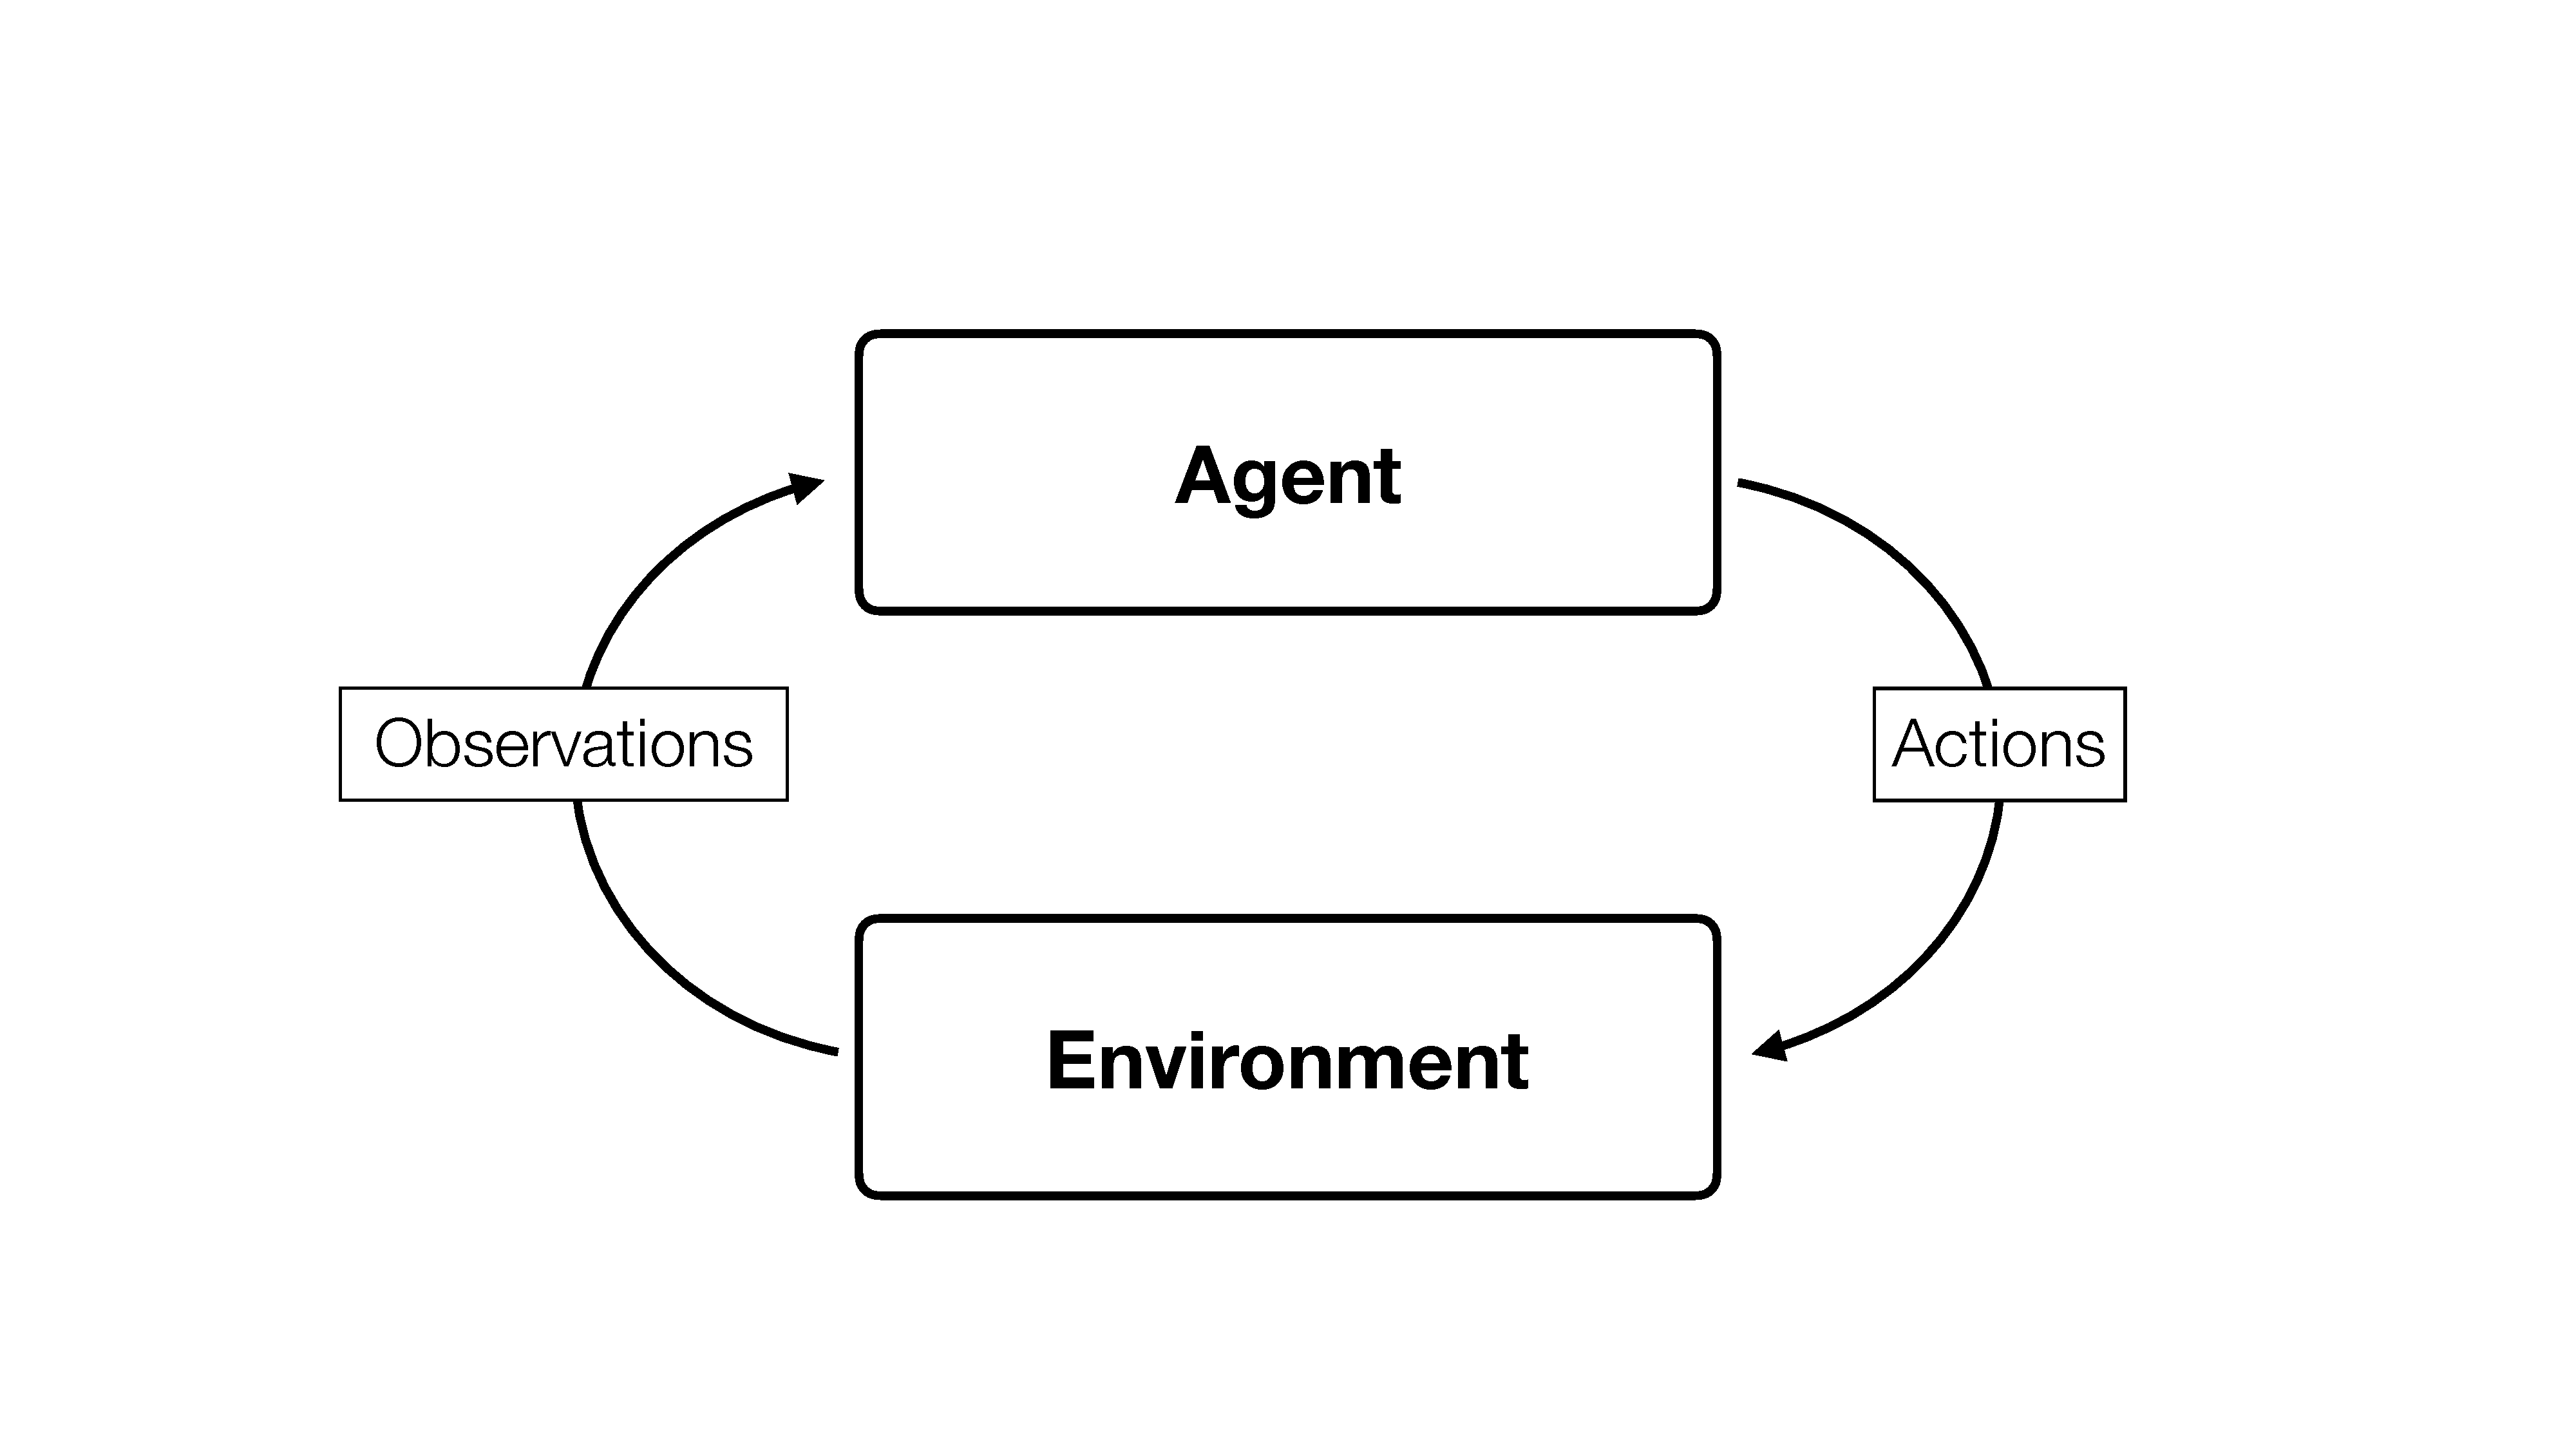
\includegraphics[width=0.6\linewidth]{./figures/intelligent_agents/env_agent_loop.pdf}
    \label{fig:env_agent_loop}
\end{figure}


\section{Imitation learning}
Imitation learning is just supervised learning applied to learning a {\bf policy}, i.e. a mapping from environment {\bf states} $s$ to actions $a$. We denote a policy as $\pi: s \rightarrow a$. Imagine we wish to learn to play chess. The imitation learning solution is to watch Gary Kasparov play the game, and learn to do exactly what he does:
\begin{figure}[h]
    \centering
    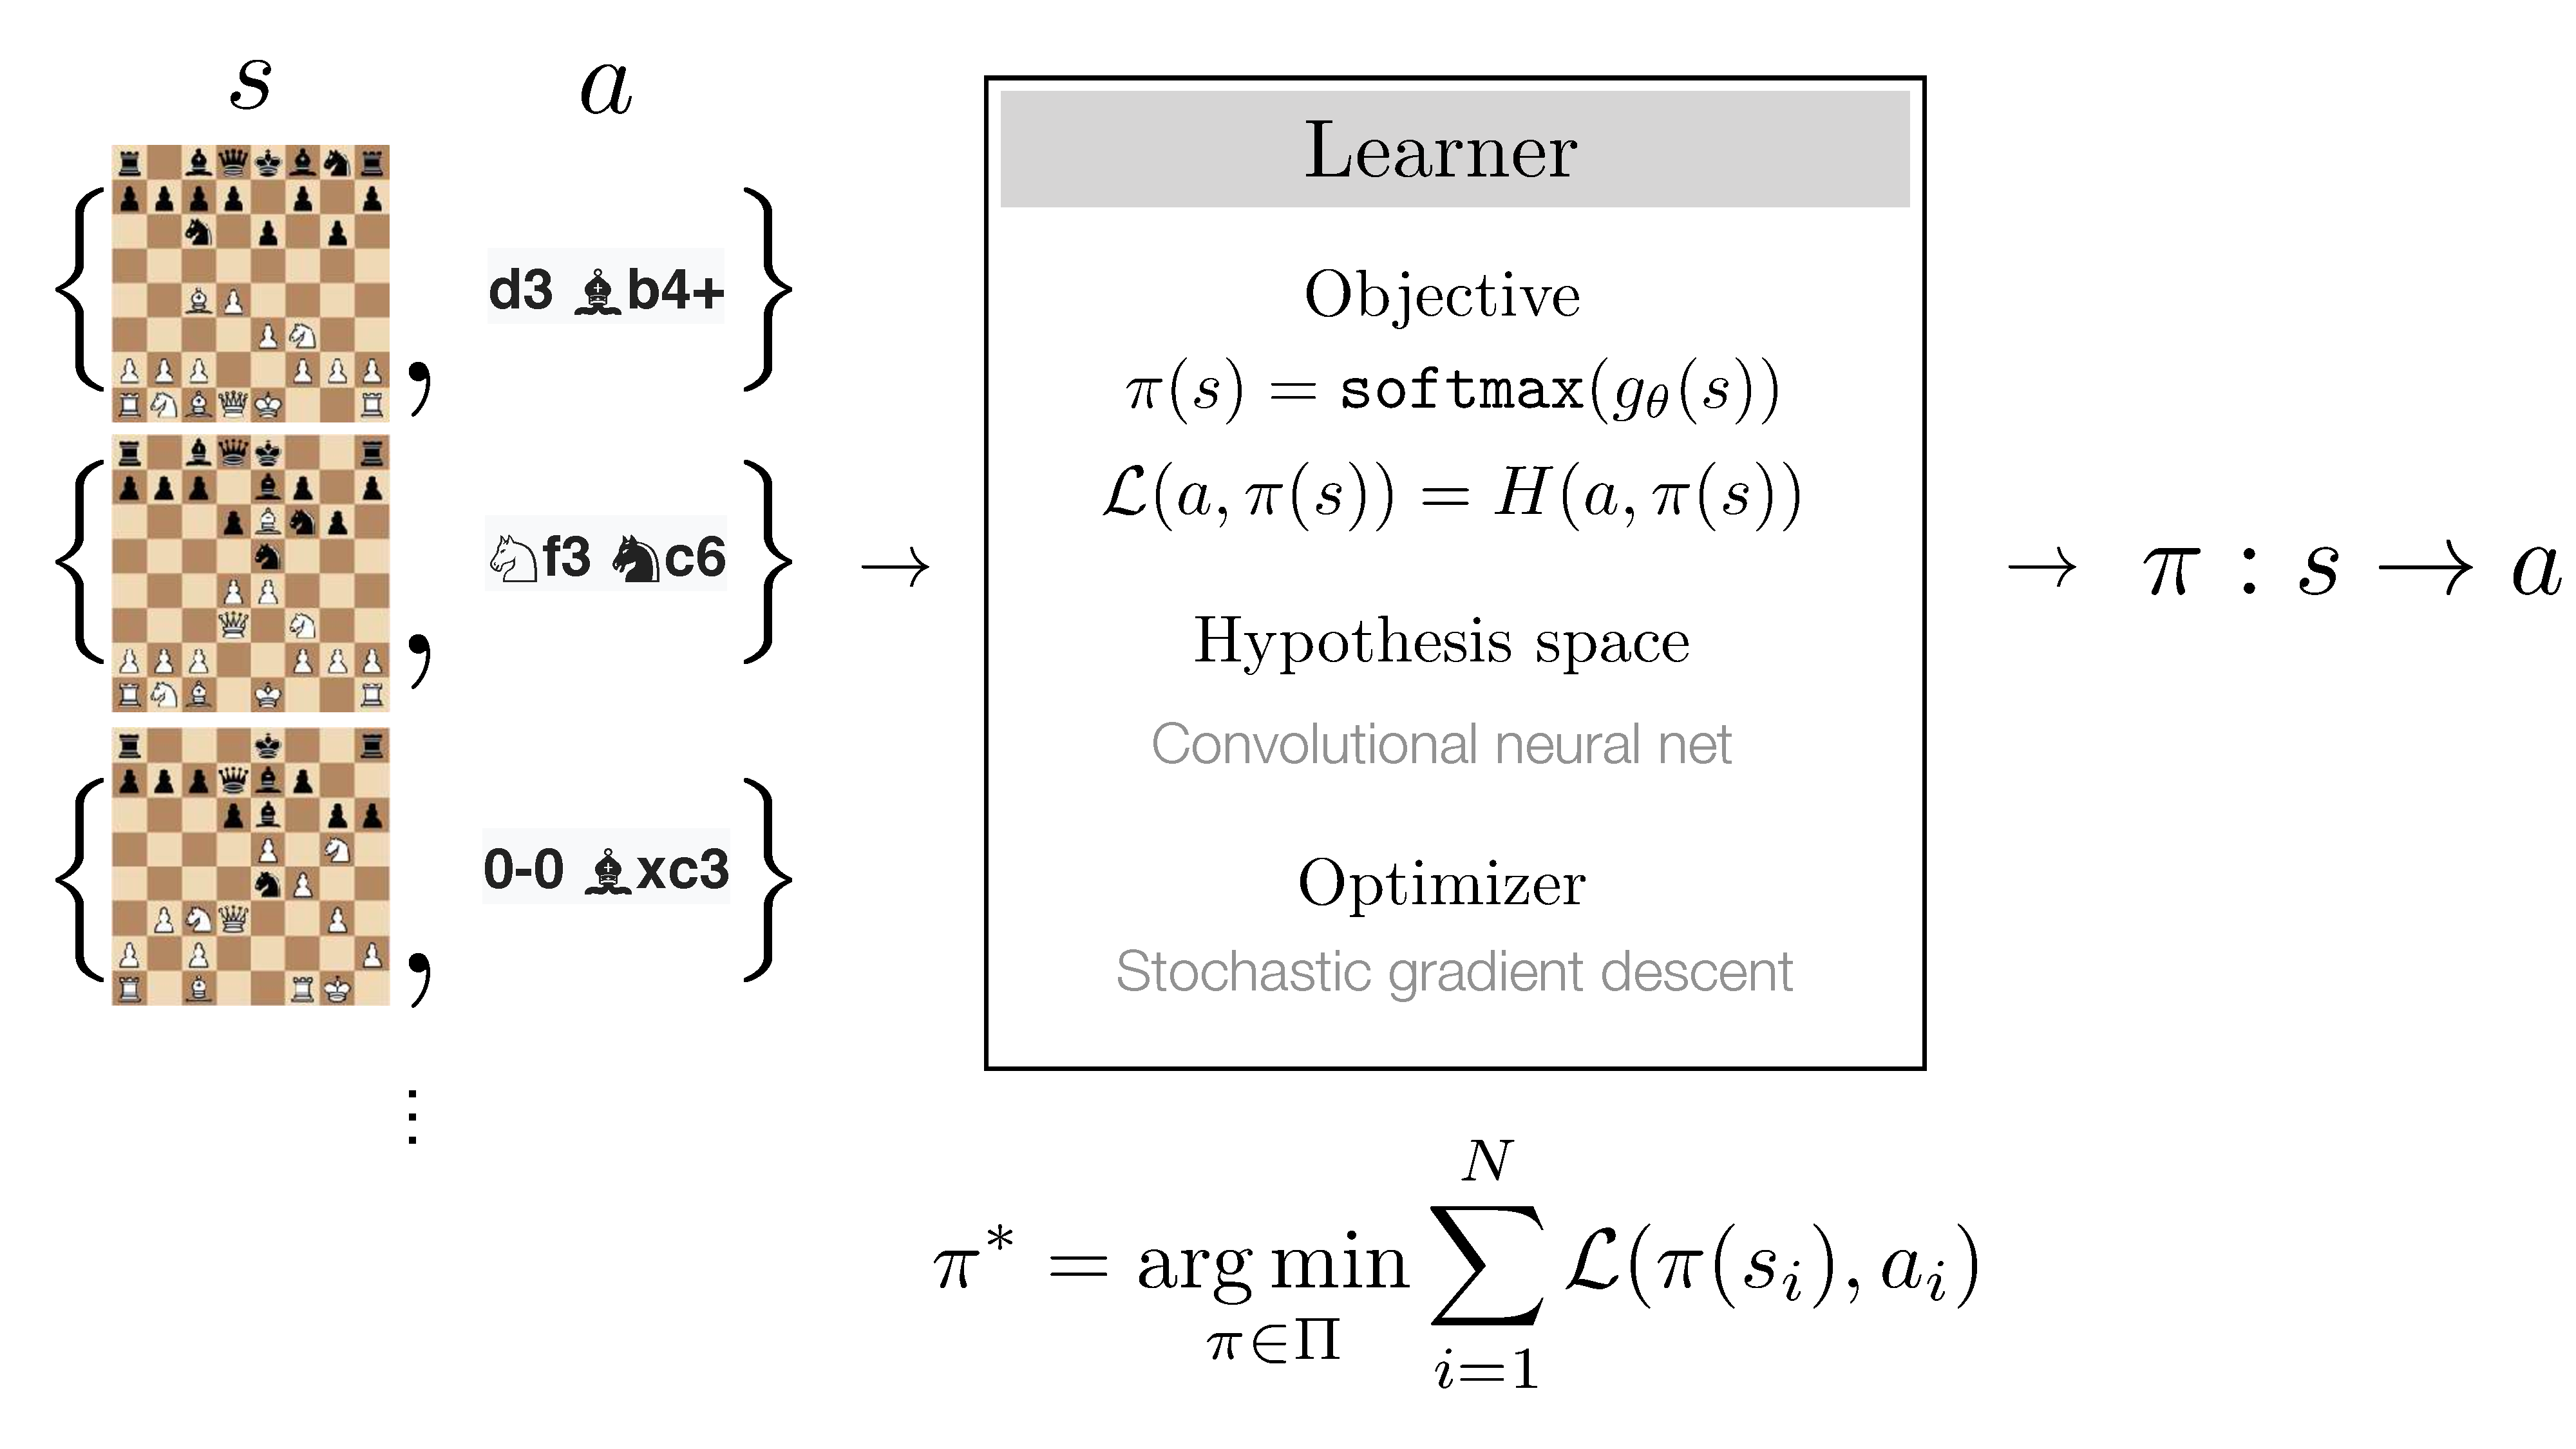
\includegraphics[width=0.8\linewidth]{./figures/intelligent_agents/imitation_learning.pdf}
    \label{fig:intelligent_agents:imitation_learning}
\end{figure}
\newpage

On the left, we have a bunch of {\bf demos} of what Kasporov did in millions of different game states. We simply train a policy that tries to match what Kasporov did whenever it encounters the same game states, or sufficiently similar ones.

\section{Reinforcement learning}
How can we learn to execute good actions if we have no expert to imitate? One answer is {\bf reinforcement learning} (RL). In RL we are only given {\bf rewards} that indicate if our behavior is good or bad, and we must {\bf explore} (i.e. try out different behaviors) to figure out which give the most positive rewards. The big difference between RL and imitation learning (a.k.a. supervised learning) is that in RL, we are not given examples (a.k.a. demos). This makes RL a much harder problem. Supervised learning is learning from examples. RL is learning by trial and error.

The basic idea of RL is actually rather intuitive: try out a bunch of behaviors, then adopt the one that led to the best outcome. For example, a chess playing agent could try out a bunch of different strategies in a tournament against human players. Maybe one strategy ends up beating all the humans. Then the agent will adopt that strategy as the one to use in future tournaments (we then say it has learned that strategy). How to do this efficiently is the central question of RL algorithms.

We can formalize the RL problem as follows. We wish to maximize the total rewards accumulated by our behavior. Behavior is defined as a {\bf trajectory} $\tau: \{s_0, a_0, r_0, s_1, a_1, r_1, \ldots\}$, which is a sequence of environment states $s_t$, actions taken $a_t$, and rewards achieved $r_t$. The policy $\pi: s_t \rightarrow a_t$ generates actions based on states. At every time step, the environment gives a reward $r_t$. This reward may be zero if nothing much has happened, positive if, e.g., we scored a point in a game, and negative if, e.g., we lost a point in a game.
The total sum of rewards over a behavioral trajectory is called the {\bf Return}, $R(\tau)$. Often we use {\bf discounted returns} to avoid infinite sums over trajectories of unbounded length:%\marginnote{Other length of the trajectory is called the {\bf horizon}.}[1.6cm]
\begin{align}
    R(\tau) = \sum_{t=0}^\infty \gamma^t r_t
\end{align}
The {\bf discount factor} $\gamma$ should be in the range $(0,1)$ so that the series doesn't diverge. You can think of $\gamma$ as how much more we care about a dollar today versus a dollar tomorrow.

Here is how the environment-agent loop looks with our notation filled in:
\begin{figure}[h]
    \centering
    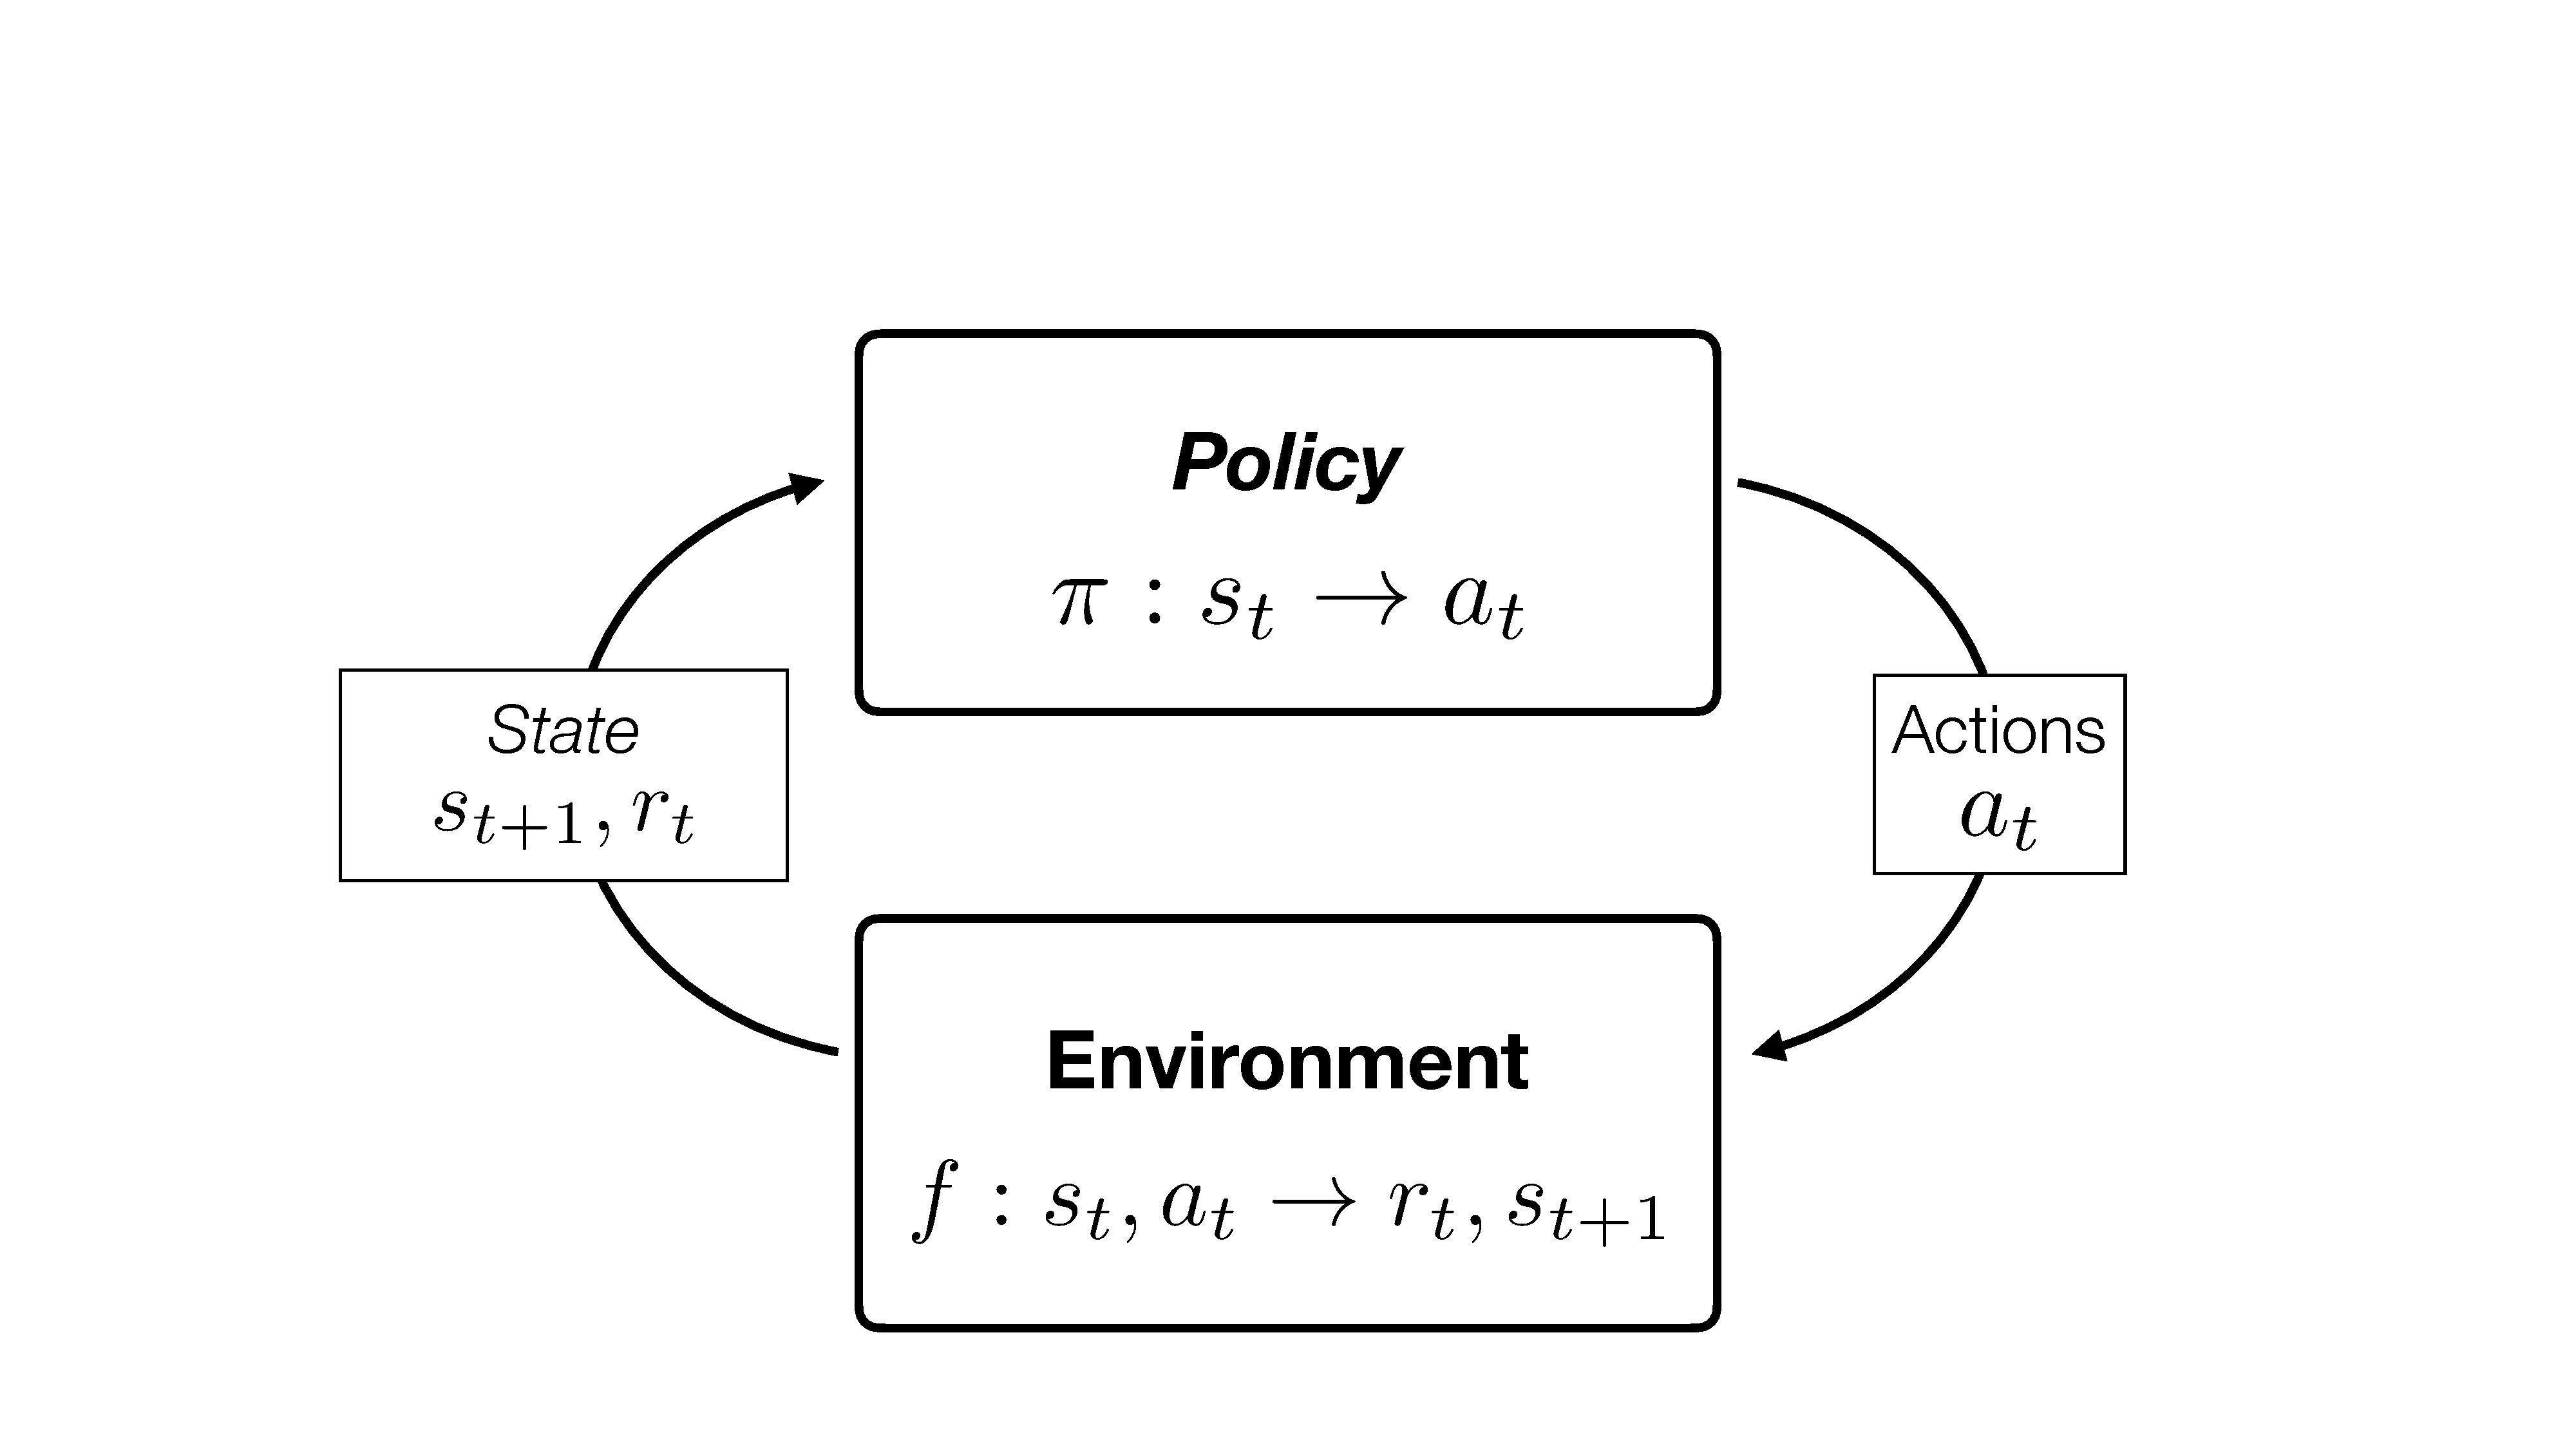
\includegraphics[width=0.6\linewidth]{./figures/intelligent_agents/env_agent_loop_with_notation.pdf}
    \label{fig:env_agent_loop_with_notation}
\end{figure}

The RL problem is to optimize the expected Returns achieved by our policy:
\begin{align}
    \pi^* &= \argmax_{\pi} \mathbb{E}_{\tau \sim \pi} [R(\tau)] \label{eqn:intelligent_agents:RL_obj}
\end{align}
Methods for performing this optimization (i.e. the \emph{optimizers} for this learning problem) include {\bf policy gradient} methods, {\bf Q learning}, {\bf genetic algorihms}, and {\bf model-based} methods.

\subsection{Markov Decision Processes}
Let's look at the expectation in Eqn. \ref{eqn:intelligent_agents:RL_obj} in more detail. What is the expectation over? The notation $\tau \sim \pi$ needs to be unpacked. In words it means ``trajectories sampled by following the policy $\pi$ in some environment $f$ starting at some initial state $s_0$." In general, we want policies that do well in many different environments with random variations, and starting from any random initial state. So the expectation could be over randomized environments and/or randomized initial states. Often we will also use a {\bf stochastic policy} that makes noisy decisions (this helps with optimization). So the expectation can also be over noise in the policy outputs. Finally, for a given environment $f$, the transition function may itself be stochastic (due to, e.g., unmodeled noise in an environment). So we can also take the expectation over noise in the transition function. When the transition function is stochastic, we may represent it with a probability distribution $P(s_{t+1} | s_t, a_t)$. The policy is another distribution, $\pi(a_t | s_t)$. The reward function can also in principle be stochastic, and in general we treat it as a function of the tuple $\{s_t, a_t, s_{t+1}\}$, so it is a distribution $r(r_t | s_t, a_t, s_{t+1})$.

In general, then, the distribution over trajectories, $\tau \sim \pi$, is modeled a {\bf Markov decision process} or {\bf MDP}, which is a graphical model with the following form:
\begin{align}
    \tau &\sim \pi\\
    \{s_0, a_0, r_0, s_1, a_1, r_1, \ldots\} &\sim \pi\\
    s_0 &\sim P(s_0) \quad\quad &&\triangleleft \text{initial state distribution}\\
    s_{t+1} &\sim P(s_{t+1} | s_t, a_t) \quad\quad &&\triangleleft \text{transition function}\\
    a_t &\sim \pi(a_t | s_t) \quad\quad &&\triangleleft \text{policy}\\
    r_t &\sim r(r_t | s_t, a_t, s_{t+1}) \quad\quad &&\triangleleft \text{reward function}
\end{align}

Visualizing this generative process as graphical model looks like this:
\begin{figure}[h]
    \centering
    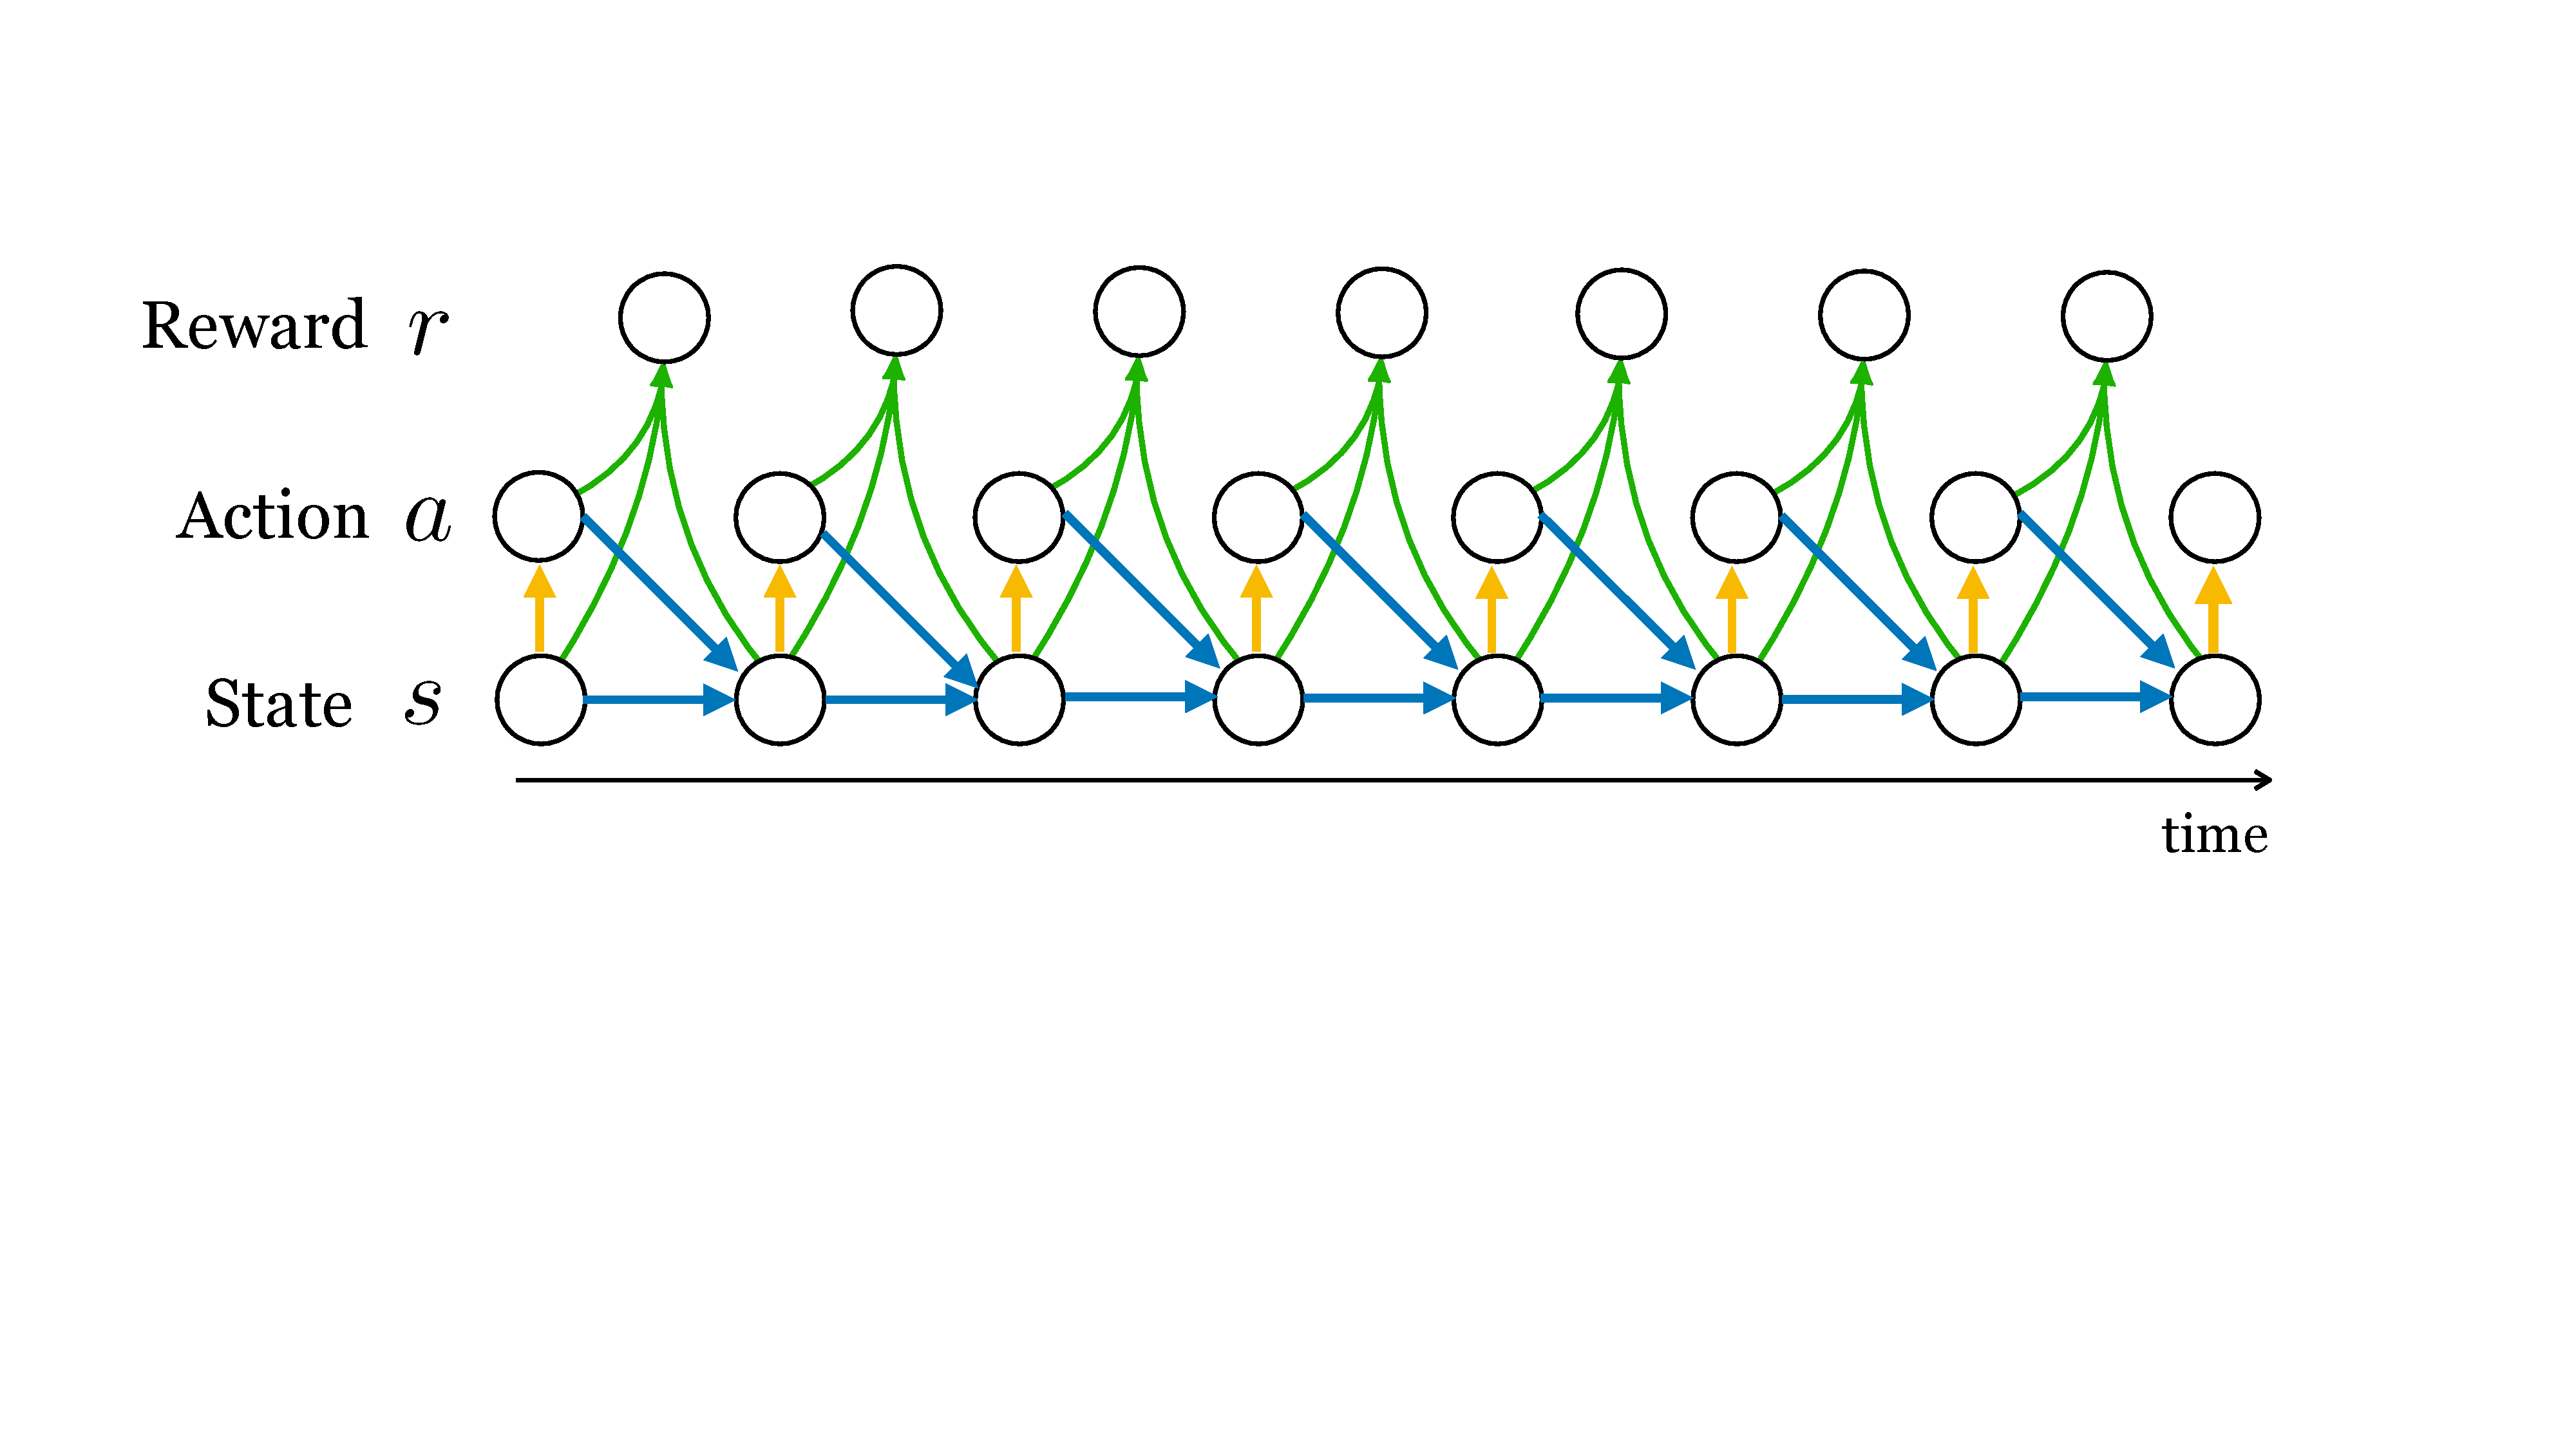
\includegraphics[width=0.8\linewidth]{./figures/intelligent_agents/MDP.pdf}
    \label{fig:intelligent_agents:MDP}
\end{figure}

The blue arrows are the environment dynamics. The green arrows are the rewards. The yellow arrows are the policy decisions. RL is the problem of learning the parameters of the yellow arrows so as the maximize the expected Return of the resulting MDP.

%World lines.

%The starting point of most RL algorithms is the observation that at any given moment, there's only one thing an agent has to decide: ``given the current state of the world, what should I do right now". 

%The agent does not have to consider how it got into it's present state -- that's in the past and you can't change the past -- and it does not have to decide exactly what it will do in the future. It just has to decide what it will do right now.

%\section{Cognitive architectures}
%Intelligent agents build \emph{representations} of their observations, use predictive mental \emph{models} to plan actions, develop compositional \emph{skills} in which multiple actions are executed in sequence, and learn intrinsic \emph{motivations} that act as surrogates for extrinsic rewards.

%Computer vision deals primarily with the first part of this pipeline: building useful representations from observations.

%\subsection{Representations}

%\subsection{Models}

%{\bf Forward dynamics models}

%{\bf Inverse dynamics models}

%\subsection{Skills}

%\subsection{Motivations}

